

\section{Introduction}\label{Introduction}
Globular clusters (\acsp{GC})\acused{GC} are self-gravitating, gas-free systems of maybe 10\(^5\) to maybe 10\(^7\) stars which are spherically grouped. There are about 150 of them in the \ac{MW}. Since they are some of the oldest stellar populations in the universe (approximately 13 Gyr), they contain much information about the assembly history and evolution of the \ac{MW}. Formerly seen as very simple spherical and isotropic stellar systems with only one stellar population, recent research revealed a much higher degree of complexity (that differ in the light-elements abundances). \acp{GC} are now known to host multiple stellar populations that challenge our understanding of their formation. Moreover, \acp{GC} now also appear dynamically complex, presenting deviations from spherical symmetry, anisotropy in velocity space and significant internal rotation.
 
\par Recent attention has been devoted to the search of \acp{IMBH} in the centre of \acp{GC}. These elusive black holes \(10^3 \mathrm{M}_\odot < \mathrm{M}_\bullet < 10^4 \mathrm{M}_\odot\) could be the missing link between stellar mass black holes (\(\mathrm{M}_\bullet < 100 \mathrm{M}_\odot\) and super massive black holes (\acsp{SMBH}, \(\mathrm{M}_\bullet > 10^5 \mathrm{M}_\odot\))\acused{SMBH} as they could represent the seed for the formation of \acp{SMBH}. Their search in the centre of \acp{GC} has partially been motivated by the extrapolation of the \(\mathrm{M}_\bullet-\sigma\)-relation for galaxies, describing the relation between the mass of a central massive black hole and the velocity dispersion of its host galaxy.
\par The hunt of \acp{IMBH} in Galactic \acp{GC} has been primarily based on two methods: 1) detection of radio and X-ray emission due to the accretion of gas in the black hole; 2) detection of kinematic signatures in the central region of a \ac{GC}. The first method proved to be difficult because the feeding of a black hole with gas is highly inefficient in a gas poor environment of Galactic \acp{GC}. 
\par The kinematic detection of \acp{IMBH} is usually based on the analysis of the velocity-dispersion profile in the inner few arcseconds around the crowded centre of a \ac{GC} in search for a rise of the dispersion. This requires a combination of high angular resolution and high spectral resolving power. For this reason the detection of \acp{IMBH} remains still highly controversial. 
\par Currently there are two different kinematic methods trying to detect \acp{IMBH}: \color{red} resolved kinematics \& unresolved integrated light [bianchini 2015] \color{black} These methods often deliver significant different results when applied to the same \ac{GC}. As an example there are the unresolved/integrated IFU kinematics which result in a signature of an \ac{IMBH} for NGC 6388 (cusp in the velocity dispersion profile) and resolved/discrete kinematics which do not yield \acp{IMBH} (no cusp in the velocity dispersion profile). \color{red} include graph of Paolo's talk!! \color{black} 
\par Given these controversial results that prevent us from drawing definite conclusions on the existence of \acp{IMBH} in Galactic \acp{GC} we propose to introduce a new approach to analyse the effects of an \ac{IMBH} to the central kinematic of a \ac{GC}. Our method consists in going beyond the traditional phase space analysis (i.e., analysis of velocity dispersion profiles), by exploiting the orbital information of the stars. Our expectation is that an \ac{IMBH} could alter the orbital properties of the stars that more closely interact with it.
\\

%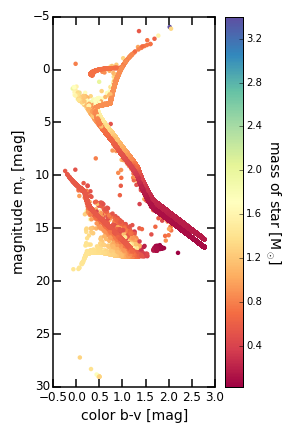
\includegraphics[width=\textwidth]{Plots/color_magnitude_diagram}
%\subsection{Orbits \& actions}
\par An orbit is a path a unperturbed, collisionless tracer particle (e.g. a star) will move along in a gravitational potential. Orbits contain information about the gravitational potential generated by the mass distribution of a system in their position and velocity coordinates following Newtons 2nd law. Orbit \acp{DF} describe which orbits are populated by how many tracers. From the orbit distribution function together with the overall potential we can draw inferences about the structure and evolution history of the system. 
\par Historically observations of orbits enabled discoveries or confirmed them: 
\begin{itemize}
\item Seen from the earth Mars' position moves over the sky as a loop called epicycle. That implies that the earth is not the centre of the universe! (C \& O p.3)
\item Neptune/Uranus \color{red} noch mal nachlesen \color{black}
\item From rotation curves of galaxies we see that stars move faster than what expected by the presence of only the mass of luminous matter. There has to be more matter interacting via gravitational forces. This has led to the theory of dark matter. (Rubin 1980)
\item Mercury's orbit differs hugely from calculated Kepler orbit. This is because of its migrating pericentre. Due to the proximity to the sun gravitational forces are so strong that we need to apply general relativity.
\item The \ac{SMBH} Sagittarius A*  was detected by observations of the orbits around the black hole and resulting mass calculations. (C \& O p.923)
\end{itemize}
\par Some examples for orbit \acp{DF} are spiral galaxies where stars of different components (thin disc, thick disc, bulge, halo) are on different orbits (dynamical distinct) and have different metallicities (chemical distinct).
\\\par Actions are integrals of motion and are the distinct description of orbits. They are constant with time. Known for a long time they are extremly difficult to calculate. Actions of our solar system can be calculated more easily since the potential is a Kepler potential. With nowadays supercomputers it is finally possible to compute actions of more complex and less explored systems.
\color{green} how to describe orbits \\ idea 1 (x(t),v(t)) pretty complicated time evolution in 6 coordinates. idea 2 take quantities which are constant with time so called integrals of motions \\ beste set von integrals of motions are actions good to interpret \color{black}
\\\par In this thesis we wish to test the feasibility of the analysis of the action/orbit space in \acp{GC} and test whether it could be possible to predict  signatures of \acp{IMBH}. This will be done by "translating" the traditional phase-space into orbit space, exploiting the potential and the \(\vec{x}\) and \(\vec{v}\) vectors. Although this type of information (6-D info) is not currently available for Galactic \acp{GC} we are motivated by the growing amount of photometric and kinematic data that are already able to deliver a 5-D info (2D spatial info and 3D kinematic info), in particular the high accuracy \ac{HST} proper motions and the upcoming GAIA data. We will limit our analysis to \ac{GC} simulations with and without \acp{IMBH} to explore our new approach. The thesis is structural in to parts: first we familiarize with a phase space analysis of the simulations and we will focus in how to study the orbits and extract predictions of the presence of an \ac{IMBH}.

